\subsection{Text strings}

\subsubsection{\CCpp}

\label{C_strings}

Die normalen C-strings sind NULL-Terminiert (\ac{ASCIIZ}-strings).

Der Grund warum C Stringformatierung so ist wie sie ist (NULL-Terminiert) scheint ein Historischer zu sein.
In [Dennis M. Ritchie, \emph{The Evolution of the Unix Time-sharing System}, (1979)] kann man nach lesen:

\begin{framed}
\begin{quotation}
Ein kleiner Unterschied war das die I/O Einheit ein ``word'' war, nicht ein Byte, weil die PDP-7 eine word-adressierte
Maschine war. In der Praxis bedeutete das lediglich das alle Programme die mit Zeichen Streams arbeiteten, das NULL 
Zeichen ignorieren mussten, weil die NULL benutzt wurde um eine Datei bis zu einer Graden Zahl an Bytes auf zu f\"ullen.

\end{quotation}
\end{framed}

\myindex{Hiew}

In Hiew oder FAR Manager sehen diese Strings so aus:

\begin{lstlisting}[style=customc]
int main()
{
	printf ("Hello, world!\n");
};
\end{lstlisting}

\begin{figure}[H]
\centering
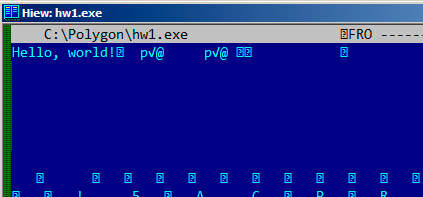
\includegraphics[width=0.8\textwidth]{digging_into_code/strings/C-string.png}
\caption{Hiew}
\end{figure}

% FIXME видно \n в конце, потом пробел

\subsubsection{Borland Delphi}
\myindex{Pascal}
\myindex{Borland Delphi}

Dem String in Passcal und Borland Delphi h\"angt eine 8 oder 32-Bit Zeichenkette an. 

Zum Beispiel:

\begin{lstlisting}[caption=Delphi,style=customasmx86]
CODE:00518AC8                 dd 19h
CODE:00518ACC aLoading___Plea db 'Loading... , please wait.',0

...

CODE:00518AFC                 dd 10h
CODE:00518B00 aPreparingRun__ db 'Preparing run...',0
\end{lstlisting}

\subsubsection{Unicode}

\myindex{Unicode}

Oft, ist das was Unicode genannt wird einfach eine Methode um Strings zu codieren, bei denen jedes Zeichen 2 Byte oder 
16 Bits verbraucht. Das ist ein h\a"ufiger Terminologischer Fehler. Unicode ist ein Standard bei dem eine Nummer 
zu einem der vielen Schreibsysteme der Welt zugeordnet wird, aber es beschreibt nicht die codierungs Methode. 

\myindex{UTF-8}
\myindex{UTF-16LE}

Die bekannteste Methode zu Codieren ist: UTF-8 ( ist weit verteilt im Internet und auf *NIX Systemen) und UTF-16LE ( wird bei Windows benutzt). 

\myparagraph{UTF-8}

\myindex{UTF-8}
UTF-8 ist eine der erfolgreichsten Methoden um Zeichen zu codieren.
Alle Latein Zeichen werden codiert so wie in ASCII, und alle Symbole nach der
ASCII Tabelle wurden codiert mit zus\"atzlichen Bytes. 0 wird codiert als davor,
also arbeiten alle Standard C String Funktionen mit UTF-8 Strings wie mit jedem anderen String auch.

Lasst uns anschauen wie die Symbole in verschiedenen anderen Sprachen nach UTF-8 Codiert werden und 
wie man sie als FAR aussehen lassen kann, durch das benutzen der codepage 437\footnote{Beispiel und \"Ubersetzung k\o"nnen von hier bezogen werden:  
\url{http://www.columbia.edu/~fdc/utf8/}}:

\begin{figure}[H]
\centering
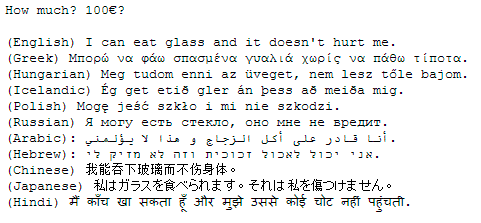
\includegraphics[width=0.8\textwidth]{digging_into_code/strings/multilang_sampler.png}
\end{figure}

% FIXME: cut it
\begin{figure}[H]
\centering
\myincludegraphics{digging_into_code/strings/multilang_sampler_UTF8.png}
\caption{FAR: UTF-8}
\end{figure}

Wie man hier sehen kann, der Englische String sieht genauso aus wie sein Gegenst\"uck in ASCII.

Die Ungarische Sprache benutzt Latein Symbole plus ein paar Symbole mit diacritic Markierungen.

Diese Symbole werden mit mehreren Bytes codiert, diese wurden rot unterstrichen.
Das gleiche gilt f\"ur die Isl\"andischen und Polnischen Sprachen.

Es gibt auch das \q{Euro} W\"ahrungs Symbol im Standard, das Symbol wurde mit 3 Bytes Codiert.

Der Rest der Schreibsysteme hat keinen Bezug zu Latein.

Zumindest in Russisch, Arabisch, Hebr\"aisch und Hindu k\"onnen wir wiederkehrende Bytes erkennen und das ist nicht mal \"uberraschend:
Alle Zeichen eines Schreibsystems werden normalerweise in der selben Unicode Tabelle angelegt, also f\"angt ihr code mit den 
immer gleichen nummern an. % <--- Wird anders \"ubersetzt.

Zu Anfang, noch vor dem \q{How much?} String sehen wir 3 Bytes, die tats\"achlich das \ac{BOM} darstellen.
Das \ac{BOM} definiert das Codierungssystem das benutzt werden soll.

\myparagraph{UTF-16LE}

\myindex{UTF-16LE}
\myindex{Windows!Win32}
Viele win32 Funktionen in Windows haben die Suffixe \TT{-A} und \TT{-W}. 
Der erste Typ Funktionen arbeitet mit normalen Strings, der andere Typ mit 
UTF-16LE Strings (\emph{wide}). 

Im zweiten Fall, wird jedes Symbol normal als 16-Bit Wert des Typs \emph{short} gespeichert.

Die Latein Symbole in UFT-16 Strings sehen in Hiew oder FAR aus als w\"aren sie mit Null Bytes verschachtelt:

\begin{lstlisting}[style=customc]
int wmain()
{
	wprintf (L"Hello, world!\n");
};
\end{lstlisting}

\begin{figure}[H]
\centering
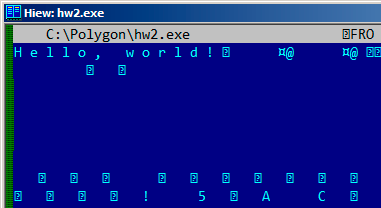
\includegraphics[width=0.8\textwidth]{digging_into_code/strings/UTF16-string.png}
\caption{Hiew}
\end{figure}

Wir k\o"nnen das oft auch in gls{Windows NT} System Dateien sehen:

\begin{figure}[H]
\centering
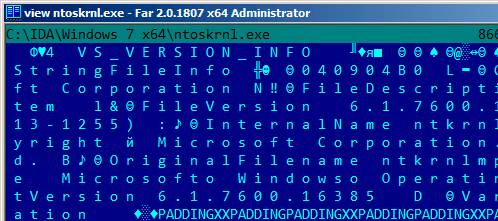
\includegraphics[width=0.8\textwidth]{digging_into_code/strings/ntoskrnl_UTF16.png}
\caption{Hiew}
\end{figure}

\myindex{IDA}
Strings mit Zeichen die exakt 2 Bytes verbrauchen werden \q{Unicode} in \IDA genannt:

\begin{lstlisting}[style=customasmx86]
.data:0040E000 aHelloWorld:
.data:0040E000                 unicode 0, <Hello, world!>
.data:0040E000                 dw 0Ah, 0
\end{lstlisting}

Hier sieht man wie Russische Sprache in UTF-16LE Codiert wird:

\begin{figure}[H]
\centering
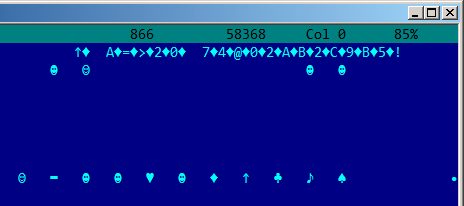
\includegraphics[width=0.8\textwidth]{digging_into_code/strings/russian_UTF16.png}
\caption{Hiew: UTF-16LE}
\end{figure}

Was man leicht sehen kann ist das die Symbole durchzogen sind von den Diamant Zeichen (das im ASCII code mit 4 codiert wird).
Tats\"achlich, findet man die Kyrillischen Symbole in der vierten Unicode Tabelle.
Deswegen, alle Kyrillischen Symbole in UTF-16LE findet man im Bereich \TT{0x400-0x4FF}.

Lass uns noch mal zu dem Beispiel gehen mit dem String der in verschiedenen Sprachen geschrieben ist.
Hier sieht man wie der String in UTF-16LE aussieht. 

% FIXME: cut it
\begin{figure}[H]
\centering
\myincludegraphics{digging_into_code/strings/multilang_sampler_UTF16.png}
\caption{FAR: UTF-16LE}
\end{figure}

Hier k\"onnen wir auch das \ac{BOM} am Anfang sehen. 
Alle Latein Zeichen enthalten Null Bytes.

Manche Zeichen mit unterschiedlichen Markierungen (Ungarisch und Isl\"andisch) wurden rot unterstrichen.

% subsection:
\subsubsection{Base64}
\myindex{Base64}

Die Base64 Codierung ist sehr weit verbreitet f\"ur f\"alle in denen man Bin\"ardaten als Textstring \"ubertragen will.

Im Grunde, codiert dieser Algorithmus 3 Bin\"ar Bytes in 4 druckbare Zeichen: 
Alle 26 Latein Zeichen (beides klein und groß Buchstaben), Ziffern, plus Zeichen (\q{+}) und slash Zeichen (\q{/}),
64 Zeichen insgesamt. 

Ein charakteristisches Feature von Base64 Strings ist das sie oft (aber nicht immer) mit 1 oder 2  \gls{padding}
Gleichheitszeichen (\q{=}) Enden, zum Beispiel: 

\begin{lstlisting}
AVjbbVSVfcUMu1xvjaMgjNtueRwBbxnyJw8dpGnLW8ZW8aKG3v4Y0icuQT+qEJAp9lAOuWs=
\end{lstlisting}

\begin{lstlisting}
WVjbbVSVfcUMu1xvjaMgjNtueRwBbxnyJw8dpGnLW8ZW8aKG3v4Y0icuQT+qEJAp9lAOuQ==
\end{lstlisting}

Das Gleichheitszeichen Symbol (q{=}) wird man niemals in der Mitte eines Base64-codierten
Strings sehen.

Jetzt ein Beispiel wie man per Hand Base64 codieren kann.
Lasst uns 0x00, 0x11 , 0x22 und 0x33 in Hexadezimalzahlen in einen Base64
String umwandeln: 

\lstinputlisting{digging_into_code/strings/base64_ex.sh}

Lasst uns alle 4 Bytes in Bin\"ar Form bringen und dann neu gruppieren in 6-Bit Gruppen:

\begin{lstlisting}
|  00  ||  11  ||  22  ||  33  ||      ||      |
00000000000100010010001000110011????????????????
| A  || B  || E  || i  || M  || w  || =  || =  |
\end{lstlisting}

Die ersten drei Bytes (0x00, 0x11, 0x22) k\"onnen in 4 Base64 Zeichen umgewandelt werden (``ABEi''),
aber nicht das letzte Byte (0x33), also wird das Byte codiert indem man zwei Buchstaben 
benutzt (``Mw'') und das \gls{padding} Symbol (``='') wird zweimal hinzugef\"ugt um die letzte
Gruppe auf 4 Zeichen zu erweitern. Das bedeutet das die L\"ange aller korrekten Base64 Strings
sich immer durch 4 Teilen l\"asst. 

\myindex{XML}
\myindex{PGP}
Base64 wird oft benutzt wenn es darum geht Bin\"ardaten in  XML Dateien zu speichern.
``Armored'' (z.B, in Text Form) PGP Cookie und Signaturen werden codiert mit Base64.

Manche Leute versuchen auch Base64 zu benutzen um Strings zu verschleiern. 
\url{http://blog.sec-consult.com/2016/01/deliberately-hidden-backdoor-account-in.html}
\footnote{\url{http://archive.is/nDCas}}.

\myindex{base64scanner}
Es gibt Werkzeuge zum scannen von beliebigen Bin\"ardateien nach Base64 Strings.
Ein solch ein Scanner ist base64scanner\footnote{\url{https://github.com/DennisYurichev/base64scanner}}.

\myindex{UseNet}
\myindex{FidoNet}
\myindex{Uuencoding}
\myindex{Phrack}
Ein weiteres Codierungssystem welches im UseNet und FidoNet sehr weit verbreitet
war, ist UUencoding. Binärdateien sind in Phrack Magazine immernoch mit UUencoding
codiert. Es hat eigentlich die gleichen Features, unterscheidet sich von Base64
jedoch insofern, dass der Dateiname auch im Header gespeichert wird.

\myindex{Tor}
\myindex{base32}
By the Way: Es gibt auch einen nahen Verwandten zu Base64: Base32., ein Alphabet das ~10 Zeichen und ~26 Latein Zeichen hat. 
Eine verbreitete Anwendung ist Onion Adressen zu codieren. 
\footnote{\url{https://trac.torproject.org/projects/tor/wiki/doc/HiddenServiceNames}},
z.B: \\
\url{http://3g2upl4pq6kufc4m.onion/}.
\ac{URL} kann keine mixed-case Latein Zeichen beinhalten, deshalb haben Tor Entwickler sich f\"ur Base32 entschieden.


